\documentclass[runningheads, a4paper]{llncs}

\usepackage{amssymb}
\setcounter{tocdepth}{3}
\usepackage{graphicx}

\usepackage{url}
\newcommand{\keywords}[1]{\par\addvspace\baselineskip
  \noindent\keywordname\enspace\ignorespaces#1}

%%%%%% Added by Wei Liu %%%%%%%
\usepackage{amsmath}
\usepackage[vlined,ruled]{algorithm2e}
\usepackage{lwdefs}
\usepackage{multirow}
%%%%%% End of Added by Wei Liu %%%%%%%


\begin{document}

\mainmatter  % start of an individual contribution

\title{Monte Carlo Expectation Maximization with Hidden Markov Models to Detect Functional Networks in Resting-State fMRI}
\author{Wei Liu, Suyash Awate, Jeffrey S. Anderson, Deborah Yurgelun-Todd, and
  P.~Thomas~Fletcher}
\institute{University of Utah}

\titlerunning{MCEM with HMM to Detect Functional Networks in fMRI}

\author{Wei Liu\inst{1} \and Suyash P. Awate\inst{1} \and Jeffrey
  S. Anderson\inst{2} \and Deborah Yurgelun-Todd\inst{3} \and P. Thomas
  Fletcher\inst{1}}

\authorrunning{Wei Liu et al.}

\institute{Scientific Computing and Imaging Institute, University of
  Utah, USA \and Department of Radiology,
  University of Utah, USA \and Department of Psychiatry, University of
  Utah, USA}

\toctitle{MCEM with HMM to Detect Functional Networks in fMRI} \tocauthor{Wei Liu \and Suyash Awate \and Jeffrey S. Anderson \and Deborah
  Yurgelun-Todd \and\\ P. Thomas Fletcher}

\maketitle


\begin{abstract}
We propose a novel Bayesian framework for partitioning the cortex into
distinct functional networks based on resting-state fMRI. Spatial
coherence within the network clusters is modeled using a hidden Markov
random field prior. The normalized time-series data, which lie on a
high-dimensional sphere, are modeled with a mixture of von
Mises-Fisher distributions. To estimate the parameters of this model,
we maximize the posterior using a Monte Carlo expectation maximization
(MCEM) algorithm in which the intractable expectation over all
possible labelings is approximated using Monte Carlo integration. We
show that MCEM solutions on synthetic data are superior to those
computed using a mode approximation of the expectation step. Finally,
we demonstrate on real fMRI data that our method is able to identify
visual, motor, salience, and default mode networks with considerable
consistency between subjects.
\end{abstract}

\section{Introduction}
Resting-state functional magnetic resonance imaging (fMRI) measures background
fluctuations in the blood oxygen level-dependent (BOLD) signal of the brain at
rest. The temporal correlations between these signals are used to estimate the
functional connectivity of different brain regions. This technique has shown
promise as a clinical research tool to describe functional abnormalities in
Alzheimer's disease, schizophrenia, and autism \cite{fox2010clinical}. In
resting-state fMRI, a standard analysis procedure is to select a region of
interest (ROI), or seed region, and find the correlation between the average
signal of the ROI and other voxels in the brain. These correlations are
thresholded so that only those voxels with significant correlations with the
seed region are shown. Recent methods to find functional networks without seed
regions include independent component analysis
(ICA)~\cite{beckmann2005tensorial}, which often includes an ad hoc method to
manually choose those components that are anatomically meaningful. Other
approaches employ clustering techniques to automatically partition the brain
into functional networks. A similarity metric is defined, e.g., correlation
\cite{5074650} or frequency coherence \cite{thirion2006detection}, and then a
clustering method such as $k$-means or spectral clustering is used to group
voxels with similar time series. A drawback of these approaches is that they
disregard the spatial position of voxels, and thus ignore the fact that
functional networks are organized into sets of spatially coherent regions.

We introduce a new data-driven method to partition the brain into networks of
functionally-related regions from resting-state fMRI. The proposed algorithm
does not require specification of a seed, and there is no ad hoc thresholding or
parameter selection. We make a natural assumption that functionally homogeneous
regions should be spatially coherent. Our method incorporates spatial
information through a Markov random field (MRF) prior on voxel labels, which
models the tendency of spatially-nearby voxels to be within the same functional
network. Each time series is first normalized to zero mean and unit norm, which
results in data lying on a high-dimensional unit sphere. We then model the
normalized time-series data as a mixture of von Mises-Fisher (vMF) distributions
\cite{banerjee2006clustering}. Each component of the mixture model corresponds
to the distribution of time series from one functional network. Solving for the
parameters in this combinatorial model is intractable, and we therefore use a
stochastic method called Monte Carlo Expectation Maximization (MCEM), which
approximates the expectation step using Monte Carlo integration. The stochastic
property of MCEM makes it possible to explore a large solution space, and it
performs better than a standard mode approximation method using iterated
conditional modes (ICM).

The proposed method in this paper is related to previous approaches using MRFs
to model spatial relationships in fMRI data. Descombes et
al.~\cite{descombes_spatio-temporal_1998} use a spatio-temporal MRF to analyze
task-activation fMRI data. Liu et al.~\cite{liu2010spatial} use an MRF model of
resting state fMRI to estimate pairwise voxel connections. However, neither of
these approaches tackle the problem of clustering resting-state fMRI into
functional networks.

\section {Hidden Markov Models of Functional Networks}\label{sec:models}
% Bayesian, prior, likelihood
We use a Bayesian statistical framework to identify functional networks of the
gray matter in fMRI data. We formulate a generative model, which first generates
a spatial configuration of functional networks in the brain, followed by an fMRI
time series for each voxel based on its network membership. We employ an MRF
prior to model network configurations, represented via unknown, or
\emph{hidden}, labels. Given a label, we assume that the fMRI time series,
normalized to zero mean and unit norm, are drawn from a von Mises-Fisher
likelihood.

% notation: indices, labels

Let $\cS = \{1, \ldots, N\}$ be the set of indices for all gray-matter
voxels. We assume that the number of networks $L$ is a known free parameter. Let
$\cL = \{1, 2, \cdots, L\}$ be the set of labels, one for each network. We
denote a label map for functionally-connected networks as a vector $\mat z =
(z_1,\dots, z_N), z_i \in \cL$.
Let $\cZ = \cL^N$ be the set of all possible $\mat z$ configurations.

\subsection{Markov Prior Model}
Functional networks should consist of few, reasonably-sized, possibly distant
regions. We model such networks $\mat z$ using the \emph{Potts}
MRF~\cite{LiBook}:
\begin{equation*}
  P(\mat z)
  =
  \frac
  {1}
  {C}
  \exp
  \Bigg(\!-\beta
  \sum_{i\in \cS}
  \sum_{j \in \cN_i}
  T (z_i \neq z_j)
  \Bigg),
\end{equation*}
where $T$ is $1$ if its argument is true and $0$ otherwise; $\cN_{i}$
is the set of neighbors of $i$ as defined by the neighborhood system
underlying the MRF; $\beta > 0$ is a model parameter controlling
label-map smoothness; $C$ is a normalization constant that is the sum
of $P(\mat z)$ over all possible configuration of $\mat z$. The
Markov-Gibbs equivalence~\cite{LiBook} implies that the conditional
distribution of $z_i$ at site $i$ is:
\begin{equation}
  \label{eq:mrfprior}
  P(z_i | \mat z_{-i})
  =
  P(z_i | z_{\cN_i})
  =
  \frac
  {
    \exp \left( -\beta \sum_{j \in \cN_i} T(z_i \neq z_j) \right)
  }
  {
    \sum_{l \in \cL} \exp \left( -\beta \sum_{j \in \cN_i}T(l \neq z_j) \right)
  },
\end{equation}
where $\mat z_{-i}$ is the collection of all variables in $\mat z$ excluding
site $i$. The neighborhood is the usual 6 adjacent voxels, which does not
overly smooth across boundaries. Previous works
\cite{wei1990monte,descombes_spatio-temporal_1998} have demonstrated the
advantages of MRF's over Gaussian smoothing in preserving segment boundaries.


\subsection {Likelihood Model}


% normalization

To make the analysis robust to shifts or scalings of the data, we normalize the
time series at each voxel to zero mean and unit length. This results in the data
being projected onto a high-dimensional unit sphere. After normalization, the
sample correlation between two time series is equal to their inner product, or
equivalently, the cosine of the geodesic distance between these two points on
the sphere. Thus, we re-formulate the problem of finding clusters of voxels with
high correlations to the problem of finding clusters with small within-cluster
distances on the sphere.

% likelihood

We use the notation $\mat x = \{ (\vec x_1, \dots, \vec x_N)\, |\,
\vec x_i \in S^{p-1} \}$ to denote the set of \emph{normalized} time
series. Observe that given $\mat z \in \cZ$, the random vectors $\vec
x_i$ are conditional independent. Thus, the likelihood $\log
P(\mat x | \mat z) = \sum_{i \in \cS} \log P (\vec x_i | z_i)$. We
model the emission function $P(\vec x_i | z_i)$ using the von
Mises-Fisher distribution
\begin{equation}
  f (\vec x_i;\vec \mu_l, \kappa_l | z_i = l)
  =
  C_p(\kappa_l)
  \exp
  \left(\kappa_l \vec \mu_l^T \vec x_i\right),
  \quad
  \vec x_i \in S^{p-1},
  \quad
  l \in {\cL}
  \label{eq:vmf}
\end{equation}
where, for the cluster labeled $l$, $\vec \mu_l$ is the mean
direction, $\kappa_l \geq 0$ is the \emph{concentration parameter},
and the normalization constant $C_p(\kappa) = {\kappa^{\frac{p}{2} -
    1}}/\{{(2\pi)^{\frac{p}{2}} I_{\frac{p}{2}-1}(\kappa)}\}$, where
$I_\nu$ denotes the modified Bessel function of the first kind with
order $\nu$. The larger the $\kappa$, the greater is the density
concentrated around the mean direction. Since \eqref{eq:vmf} depends
on $\vec x$ only by $\vec \mu^T \vec x$, the vMF distribution is
unimodal and rotationally symmetric around $\vec \mu$.

% 'prior' on kappa

In the Bayesian framework, we also define distributions on parameters. We assume
that $\forall l \in \cL$, $\kappa_l \sim \cN(\mu_{\kappa}, \sigma_{\kappa}^2)$
with hyperparameters $\mu_{\kappa}$ and $\sigma_{\kappa}^2$ that can be set
empirically. This prior enforces constraints that the clusters should not have
extremely high or low concentration parameters. We empirically tune the
hyperparameters $\mu_{\kappa}$ and $\sigma_{\kappa}^2$ and have found the results to be
robust to specific choices of the hyperparameters. 


\section{Monte Carlo EM}
\label{sec:mcem}


To estimate the model parameters and the hidden labels, we use a
stochastic variant of expectation maximization (EM) called Monte Carlo
EM (MCEM)~\cite{wei1990monte}. The standard EM algorithm maximizes the
expectation of the log-likelihood of joint pdf of $\mat x$ and the
hidden variable $\mat z$ with respect to the posterior probability
$P(\mat z | \mat x)$, i.e. $\mathbb{E}_{P(\mat z| \mat x)} [\log
  P(\mat x, \mat z; \vec \theta)]$. The combinatorial number of
configurations for $\mat z$ makes this expectation intractable. Thus, we
use Monte Carlo simulation to approximate this expectation as
\begin{equation}
  \widetilde Q(\vec \theta; \mat x, \mat z)
  \approx
  \frac
  {1}
  {M}
  \sum_{m=1}^{M}
    \log
    P (\mat z^m; \beta)
    +
    \log
    P (\mat x | \mat z^m; \vec \theta_L),
  \label{eq:mcemq}
\end{equation}
where $\mat z^m$ is a sample from $P(\mat z | \mat x)$, $\vec \theta_L = \{\vec
\mu_l, \kappa_l : l \in \cL\}$ is the parameter vector of the likelihood, and
$\vec \theta=\{\beta, \vec \theta_L\}$ is the full parameter vector of the
model. Computing the MRF prior in \eqref{eq:mcemq} is still intractable due to
the normalization constant, and we instead use a pseudo-likelihood
approximation~\cite{LiBook}, which gives
\begin{align*}
\centering
  \widetilde Q
  &
  \approx
  \frac{1}{M}
  \sum_{m=1}^{M}
  \sum_{i \in \cS}
  \log P(z_i | z_{\cN_i}; \beta)
  +
  \frac{1}{M}
  \sum_{m=1}^{M}
  \sum_{i \in \cS}
  \log
  P(\vec x_i | z_i; \vec \theta_L)
  =
  \widetilde Q_P
  +
  \widetilde Q_L.
\end{align*}
We use $\widetilde Q_P$ to denote the log-pseudo-likelihood of the prior
distribution, and use $\widetilde Q_L$ to denote the log-likelihood
distribution.


\subsection{Sampling from the Posterior}


Given the observed data $\mat x$ and parameter value $\vec \theta =
\{\beta, \vec \theta_L \}$, we sample from the posterior
distribution $P(\mat z | \mat x; \vec \theta)$ using Metropolis
sampling. We define the posterior energy, which is to be minimized, as the
negative log of the posterior $P(z_i | \vec x_i)$. Thus,
Bayes rule implies:
\begin{equation}
  U( z_i = l| \mat x)
  =
   \beta \sum_{j \in \cN_i} T(z_i \neq z_j)
    -
    \log C_p(\kappa_l)
    -
    \kappa_l \vec \mu_l^T \vec x_i
  + \mathrm{const},
  \label{eq:sample}
\end{equation}
which is the sum of the prior energy, the conditional energy, and a
parameter-independent quantity. Then, given a current configuration
$\mat z^n$ Metropolis sampling generates a new candidate label map $\mat w$ as
follows: (i) draw a new label $l'$ at site $i$ with uniform
distribution; $\mat w$ has value $l'$ at site $i$, with other sites
remaining the same as $\mat z^n$; (ii) compute the change of energy
$\Delta U(\mat w) = U(\mat w | \mat x) - U( \mat z^n | \mat x) = U(z_i
= l'| \mat x) - U(z_i = l | \mat x)$; (iii) accept candidate $\mat w$
as $\mat z^{n+1}$ with probability $\min (1, \exp \{ -\Delta U(\mat w)
\})$; (iv) after a sufficiently long burn-in period, generate a sample of size $M$
from the posterior distribution $P(\mat z| \mat x)$.


\subsection{Parameter Estimation}


\textbf {Estimating $\vec \theta_L$:} By maximizing $\widetilde Q_L$
with the constraint $\norm{\vec \mu_l} = 1$, we get
\begin{equation}
  R_l = \sum_{m=1}^{M}\sum_{i \in \cS_l}^{} \vec x_i, \qquad \hat {\vec \mu}_l = \frac{R_l}{\norm{R_l}},
  \label{eq:mlmu}
\end{equation}
where $S_l = \{ i \in \cS: z_i = l\}$ is the set of data points in cluster
$l$. We have no \emph{a priori} knowledge for $\vec \mu_l$, so a maximum
likelihood estimation in \eqref{eq:mlmu} is the best we can do. For $\kappa_l$
we
maximize the posterior distribution $P(\kappa_l | \mat x, \mat z^1, \dots, \mat
z^M) $.  Since $\widetilde Q_L$ is not dependent on $\kappa$, we
maximize $\widetilde Q_L(\kappa_l) + \log P(\kappa_l; \mu_{\kappa},
\sigma_{\kappa}^2)$ and get
\begin{equation}
  A_p(\hat \kappa_l) + \frac{\hat \kappa_l - \mu_{\kappa}}{N_l\sigma_{\kappa}^2} = R_l,
  \label{eq:estkappa}
\end{equation}
where $A_p(\hat \kappa_l) = I_{\frac{p}{2}} (\hat \kappa_l) / I_{\frac{p}{2}-1}
(\hat \kappa_l)$ and $N_l = |\cS_l|$ is the number of data points in cluster
$l$. Because \eqref{eq:estkappa} contains the ratio of two modified Bessel
functions, an analytic solution is unavailable and we have to resort to a
numerical solution. We use Newton's method for solving $g(\hat \kappa_l) =
A_p(\hat \kappa_l) -(\hat \kappa_l - \mu_{\kappa}) / (N_l\sigma_{\kappa}^2) -
R_l= 0$. The choice of initial value for Newton's algorithm depends on the
strength of the prior on $\kappa_l$ (i.e. the $\sigma_{\kappa}$ value). For a
noninformative prior, $\hat \kappa_l = (pR_l - R^3) / (1 - R^2)$ is a good a
good initial value \cite{banerjee2006clustering}. For a strong prior, a
reasonable initial value is the current value of $\kappa_l$.

\textbf{Estimating $\beta$:} To estimate $\beta$, we again rely on Newton's method
to find the solution numerically. The derivatives $\partial \widetilde Q_P
/ \partial \beta$ and $\partial^2 \widetilde Q_P / \partial \beta^2$ for the
pseudo-likelihood approximation of the MRF prior are easily computed.

%% \begin{algorithm}[hbt]
%%   % \DontPrintSemicolon
%%   \SetKwInOut{Input}{input}\SetKwInOut{Output}{output}
%%   \Input{Preprocessed 4D fMRI data; number of clusters}
%%   \Output{Labeled functional network map}

%%   Initialization: Run $k$-means clustering a few times and choose $\mat z$ with the smallest sum-of-square errors; estimate $\vec \theta_L$ and set
%%   $\beta$ to a small value\;

%%   \While{MCEM not converged}{
%%     \textbf{E step: } Given current $\vec \theta$,
%%     \For{$m \leftarrow 1$ \KwTo $M$}{
%%       \lForEach{$i \in \cS$} {
%%         Draw sample $z_i^m$ from $P( z_i|\mat x)$ using \eqref{eq:sample}\;
%%       }
%%     }
%%     \textbf{M step: } Given $(\mat z^1,\dots, \mat z^M)$, estimate $\beta$ and $\vec \theta_L$\;
%%     Estimate labels with ICM, using the current estimates for $\beta$ and $\vec \theta_L$ \;
%%   }

%%   \caption{MCEM-ICM Algorithm for Hidden-MRF Model Estimation}
%%   \label{alg:mcem}
%% \end{algorithm}

\subsection{MCEM-Based Algorithm for Hidden-MRF Model Estimation}

Given the methods for sampling and parameter estimation, we estimated
the hidden-MRF model by iteratively using (i) MCEM to learn model
parameters and (ii) using ICM to compute optimal network labels. In the
expectation (E) step, we draw samples from the posterior $P(\mat z |
\mat x)$, given current estimates for parameters $\vec \theta$. In the
maximization (M) step, we use these samples to update estimates for
the parameters $\vec \theta$.

\begin{figure}[!t]
  \centering
  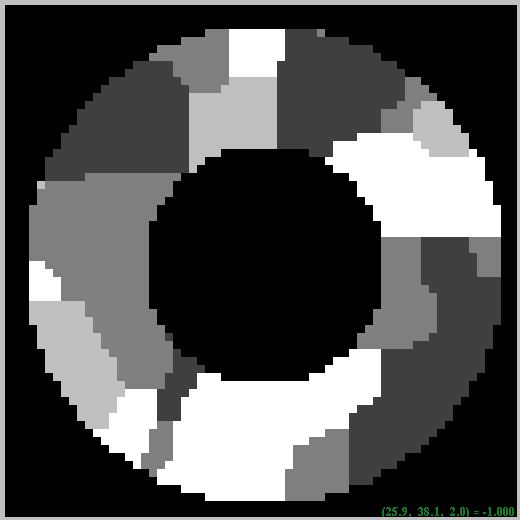
\includegraphics[width=0.19\textwidth]{figures/synthetic/true}
  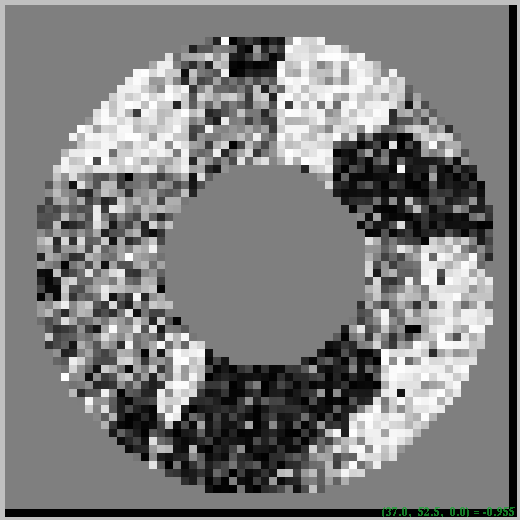
\includegraphics[width=0.19\textwidth]{figures/synthetic/obs}
  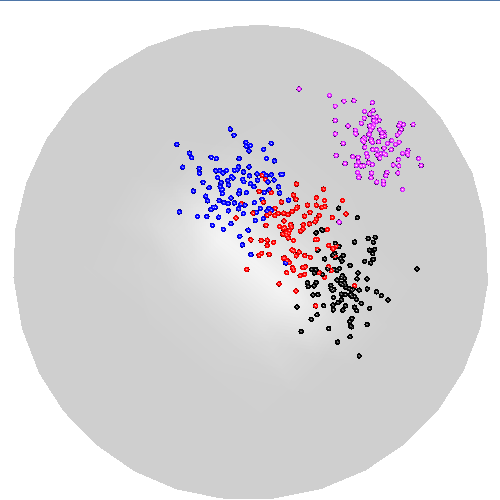
\includegraphics[width=0.19\textwidth]{figures/synthetic/sphere1}
  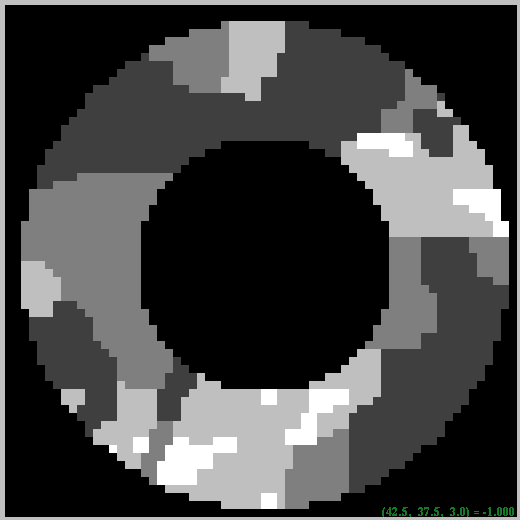
\includegraphics[width=0.19\textwidth]{figures/synthetic/label_icm}
  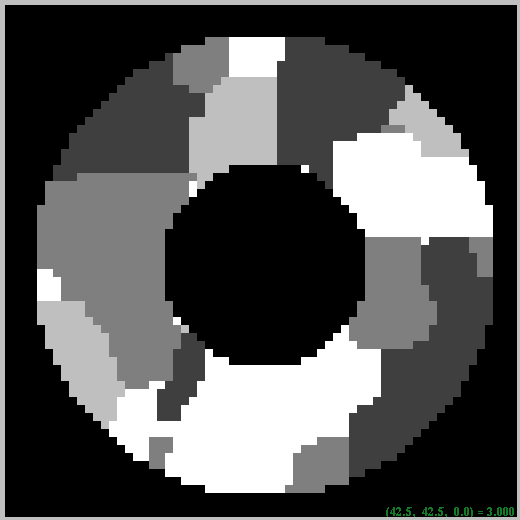
\includegraphics[width=0.19\textwidth]{figures/synthetic/label_mc}
  \caption{Synthetic example. From left to right: true labels, first
    time point of observed time series, time series plot on sphere,
    label map estimated by mode-approximation, and label map estimated by MCEM.}
  \label{fig:toy}
\end{figure}


\section{Results and Conclusion}
\label{sec:exp}


\textbf{Synthetic example:} We first simulate low-dimensional time series (2D
64$\times$64 image domain; 3 timepoints, for visualization on sphere $S^2$) to
compare the (i)~proposed method using MCEM with (ii)~the mode-approximation
approach that replaces the E step in EM with a mode approximation. We simulate a
label map by sampling from a MRF having $\beta = 2$. Given the label map, we
simulate vMF samples (on the sphere $S^2$). Figure~\ref{fig:toy} shows that the
MCEM solution is close to the ground truth, while the mode-approximation
solution is stuck in a local maximum.

\noindent{\bf Resting-State fMRI:} We evaluated the proposed method on real
data, from healthy control subjects, in a resting-state fMRI study. BOLD EPI
images (TR = 2.0 s, TE = 28 ms, 40 slices at 3 mm slice thickness, 64 x 64
matrix, 240 volumes) were acquired on a Siemens 3 Tesla Trio scanner. The
data was preprocessed in SPM, including motion correction,
registration to T2 and T1 structural MR images, spatial smoothing by a Gaussian
filter, and masked to include only the
gray-matter voxels. We used the \texttt{conn} software~\cite{connwebsite} to
regress out signals from the ventricles and white matter, which have a high
degree of physiological artifacts. A bandpass filter was used to remove
frequency components below 0.01 Hz and above 0.1 Hz. We then projected the data
onto the unit sphere by subtracting the mean of each time series and dividing by
the magnitude of the resulting time series. We then applied the proposed method
to estimate the functional network labels with the number of clusters set to $L = 8$.


Figure~\ref{fig:wholebrain} shows the optimal label maps, produced by the
proposed method for 3  of all 16 subjects in the dataset. We note that among the 8 clusters, one
cluster, with the largest $\kappa$ value and largest number of voxels,
corresponds to background regions with weakest connectivity and is not shown in
the figure. Among the clusters shown, we can identify the visual, motor, dorsal
attention, executive control, salience, and default mode
networks (DMN)~\cite{raichle2001}. Four networks: the visual, motor, executive
control, and DMN, were robustly found across all subjects. More
variability was found in the dorsal attention network (notice that it is much
larger in subject 3) and salience network (notice that it is missing in subject
2). We found that changing the number of clusters, although leading to different
label maps, preserves the four robust networks. For instance, we also ran the
analysis with the number of clusters set to 4 or 6 (results not shown) and were
able to recover the same four robust networks.

\begin{figure}[!t]
 \begin{center}
 \begin{tabular}{cccccc}
      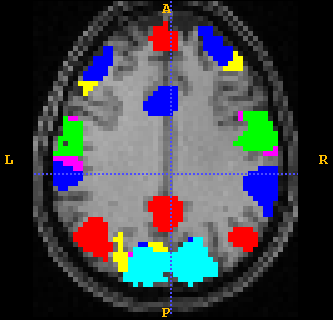
\includegraphics[width=0.15\textwidth]{figures/wholebrain/sub1/axial0028} &
      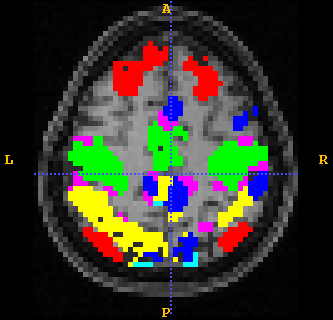
\includegraphics[width=0.15\textwidth]{figures/wholebrain/sub1/axial0034} &
      \vspace{0.5pt}
      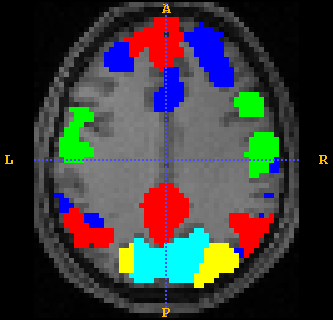
\includegraphics[width=0.15\textwidth]{figures/wholebrain/sub2/axial0028} &
      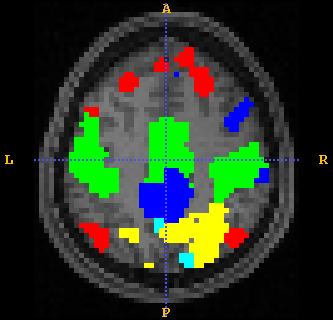
\includegraphics[width=0.15\textwidth]{figures/wholebrain/sub2/axial0034} &
      \vspace{0.5pt}
      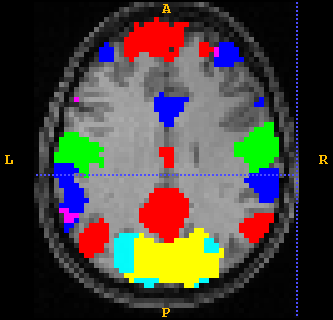
\includegraphics[width=0.15\textwidth]{figures/wholebrain/sub5/axial0028} &
      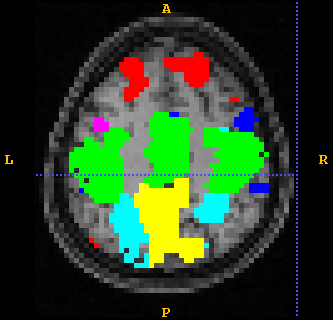
\includegraphics[width=0.15\textwidth]{figures/wholebrain/sub5/axial0034} \\

      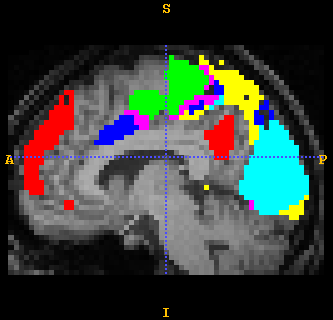
\includegraphics[width=0.15\textwidth]{figures/wholebrain/sub1/saggital0029} &
      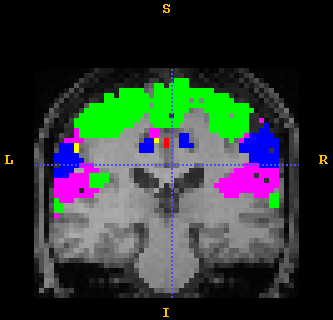
\includegraphics[width=0.15\textwidth]{figures/wholebrain/sub1/coronal0029} &
      \vspace{0.5pt}

      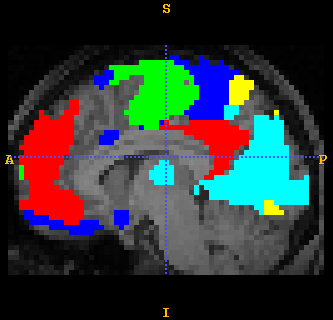
\includegraphics[width=0.15\textwidth]{figures/wholebrain/sub2/saggital0029} &
      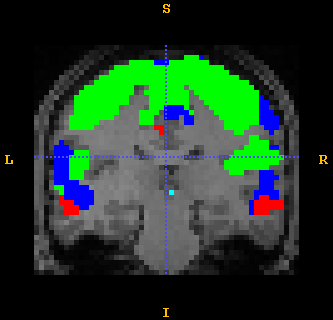
\includegraphics[width=0.15\textwidth]{figures/wholebrain/sub2/coronal0029} &
      \vspace{0.5pt}
      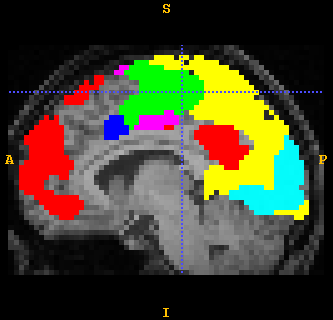
\includegraphics[width=0.15\textwidth]{figures/wholebrain/sub5/saggital0029} &
      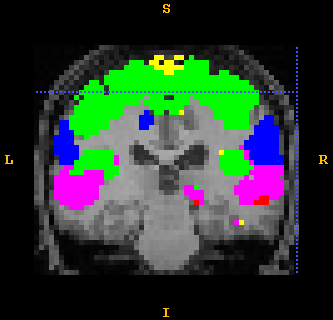
\includegraphics[width=0.15\textwidth]{figures/wholebrain/sub5/coronal0029}\\

      \multicolumn{2}{c}{Subject 1} &
      \multicolumn{2}{c}{Subject 2} &
      \multicolumn{2}{c}{Subject 3}
    \end{tabular}
  \end{center}
  \caption {Functional networks detected by the proposed method for 3 subjects
    overlaid on their T1 images.  The clusters are the visual (cyan), motor
    (green), executive control (blue), salience (magenta), dorsal attention
    (yellow), and default mode (red) networks.}
  \label{fig:wholebrain}
\end{figure}

\begin{table}[bh]
  \centering
  \caption{The number of voxels with value greater than 8 in the overlapped label map. }
  \begin{tabular*}{0.75\textwidth}{@{\extracolsep{\fill}} l  r r r r}
    & DMN & Motor & Attention & Visual \\
    \hline
    MCEM    & 5043  & 7003 & 3731 & 5844 \\
    Individual ICA & 114 & 167 & 228 & 134 \\
    Group ICA & 3075 & 5314 & 3901 & 3509
  \end{tabular*}\label{table:agreement}
\end{table}

The next experiment compares our results with ICA. A standard ICA toolbox (GIFT;
\url{mialab.mrn.org}) was applied on the same preprocessed data of each subject
independently, which we call ``Individual ICA''. We also applied standard Group
ICA, using all data from the 16 subjects simultaneously. In both ICA experiments
the number of components are set to 16. The component maps are converted to z
score and thresholded at 1. For each method we computed an overlap map for each
functional network by adding the corresponding binary label maps of all 16 subjects.
The results in Figure~\ref{fig:multisub} show our method can detect the motor,
attention, and visual network with accuracy comparable with Group ICA. Besides,
our method also detects DMN with posterior cingulate cortex (PCC) and medial
prefrontal cortex (MPFC), while Group ICA split the DMN into two components, one
with the MPFC and another with the PCC (not shown).

To see the consistency of the label map between subjects for all three methods,
we look at each method's overlapped label map and count the number of voxels
whose value are greater than 8. Table~\ref{table:agreement} shows that our
method exhibits better consistency than both Individual and Group ICA.

\begin{figure}[!t]
  \begin{center}
    \begin{tabular}{cccccccc}

      \multicolumn{2}{c}{DMN} &
      \multicolumn{2}{c}{Motor} &
      \multicolumn{2}{c}{Attention} &
      \multicolumn{2}{c}{Visual}\\

      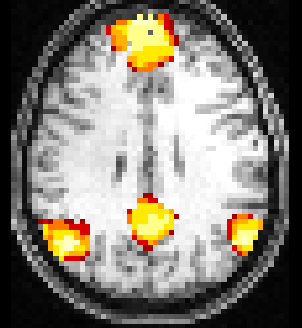
\includegraphics[height=0.10\textwidth]{figures/workshop/mcem/dmn_a} &
      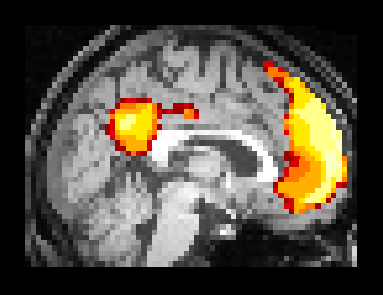
\includegraphics[height=0.10\textwidth]{figures/workshop/mcem/dmn_s} &
      \vspace{1pt}
      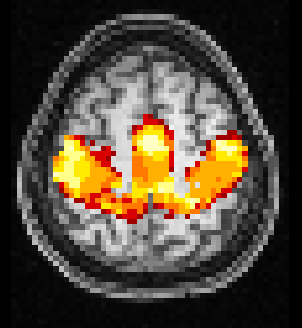
\includegraphics[height=0.10\textwidth]{figures/workshop/mcem/motor_a} &
      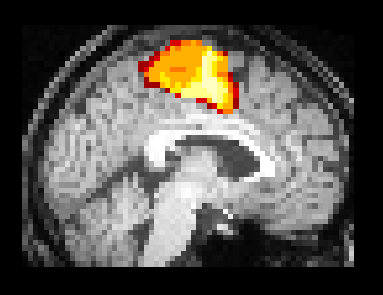
\includegraphics[height=0.10\textwidth]{figures/workshop/mcem/motor_s} &
      \vspace{1pt}
      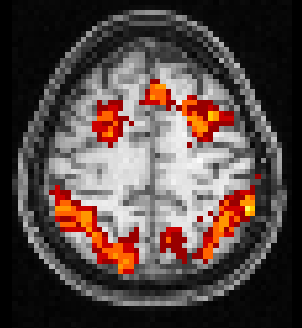
\includegraphics[height=0.10\textwidth]{figures/workshop/mcem/atten_a} &
      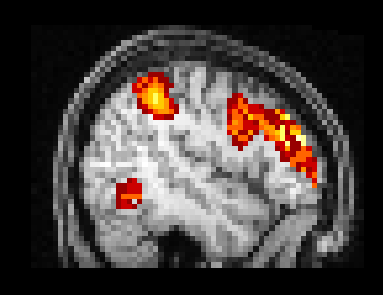
\includegraphics[height=0.10\textwidth]{figures/workshop/mcem/atten_s} &
      \vspace{1pt}
      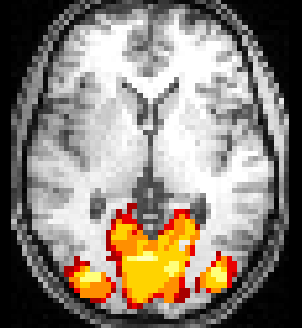
\includegraphics[height=0.10\textwidth]{figures/workshop/mcem/visual_a} &
      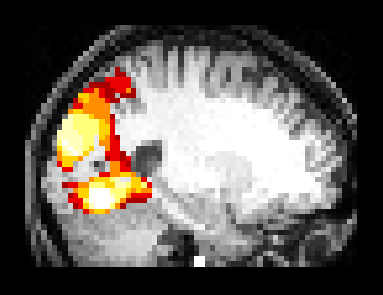
\includegraphics[height=0.10\textwidth]{figures/workshop/mcem/visual_s} \\
      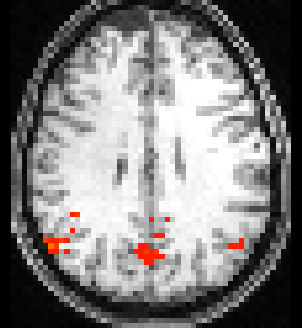
\includegraphics[height=0.10\textwidth]{figures/workshop/ica_separate/DMN_a} &
      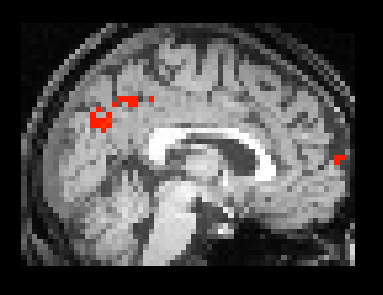
\includegraphics[height=0.10\textwidth]{figures/workshop/ica_separate/DMN_s} &
      \vspace{1pt}
      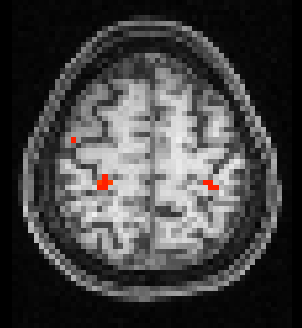
\includegraphics[height=0.10\textwidth]{figures/workshop/ica_separate/motor_a} &
      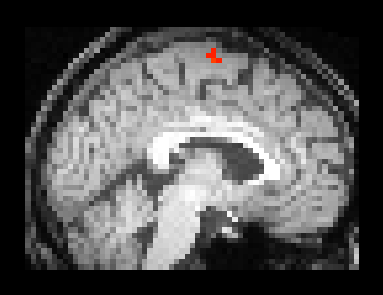
\includegraphics[height=0.10\textwidth]{figures/workshop/ica_separate/motor_s} &
      \vspace{1pt}
      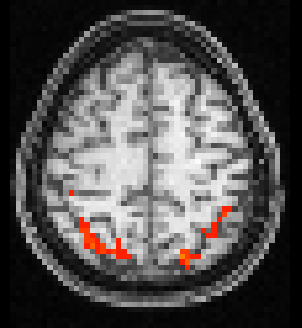
\includegraphics[height=0.10\textwidth]{figures/workshop/ica_separate/atten_a} &
      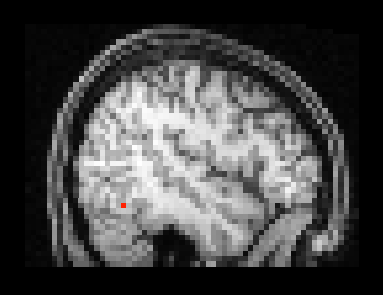
\includegraphics[height=0.10\textwidth]{figures/workshop/ica_separate/atten_s} &
      \vspace{1pt}
      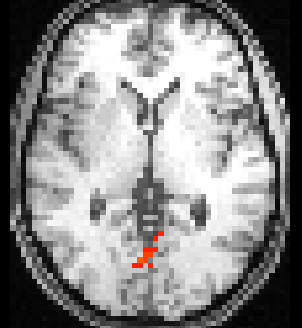
\includegraphics[height=0.10\textwidth]{figures/workshop/ica_separate/visual_a} &
      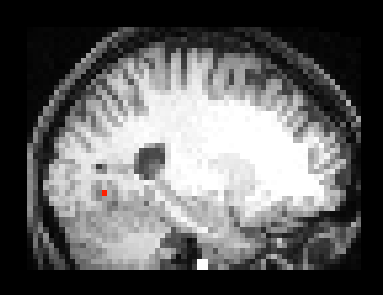
\includegraphics[height=0.10\textwidth]{figures/workshop/ica_separate/visual_s} \\
      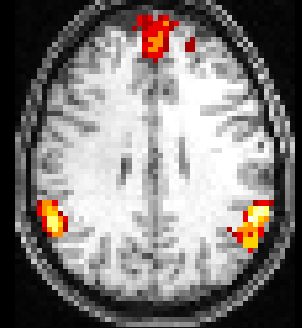
\includegraphics[height=0.10\textwidth]{figures/workshop/ica_single/dmn_a} &
      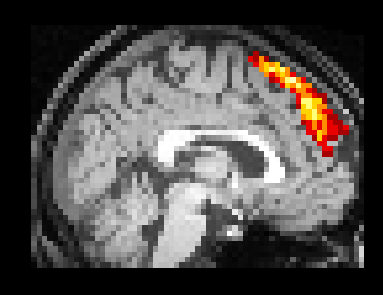
\includegraphics[height=0.10\textwidth]{figures/workshop/ica_single/dmn_s} &
      \vspace{1pt}
      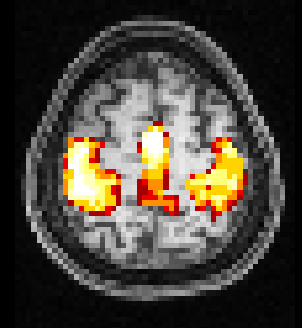
\includegraphics[height=0.10\textwidth]{figures/workshop/ica_single/motor_a} &
      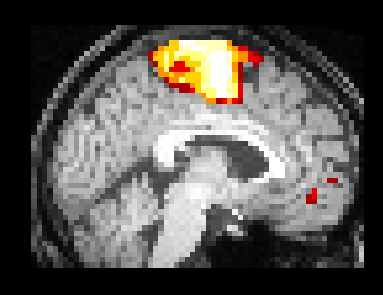
\includegraphics[height=0.10\textwidth]{figures/workshop/ica_single/motor_s} &
      \vspace{1pt}
      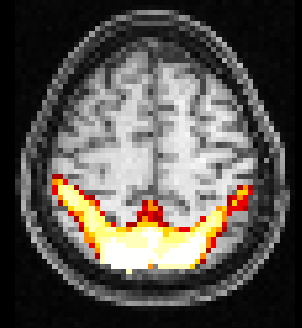
\includegraphics[height=0.10\textwidth]{figures/workshop/ica_single/atten_a} &
      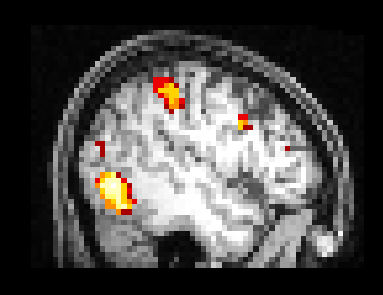
\includegraphics[height=0.10\textwidth]{figures/workshop/ica_single/atten_s} &
      \vspace{1pt}
      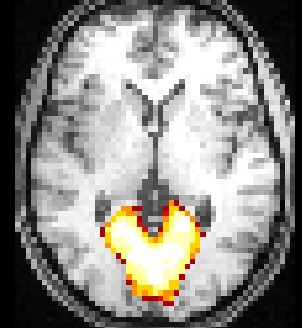
\includegraphics[height=0.10\textwidth]{figures/workshop/ica_single/visual_a} &
      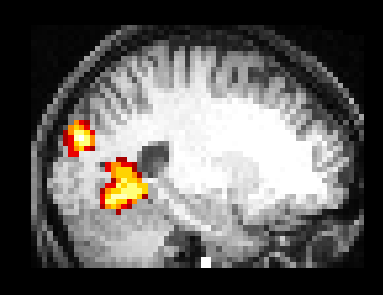
\includegraphics[height=0.10\textwidth]{figures/workshop/ica_single/visual_s} 
    \end{tabular}
  \end{center}
  \caption{Comparison of overlap label maps by our approach and ICA for 16
    subjects. Top: our MCEM approach, middle: Individual ICA, bottom: Group
    ICA. Color ranges from 8 (red) to 16 (yellow).}
  \label{fig:multisub}
\end{figure}


\noindent\textbf{Conclusion: } We present a novel Bayesian approach to detect
functional networks of the brain from resting-state fMRI that incorporates an
MRF for spatial regularization, and we use MCEM to approximate the maximum
posterior solution. Future work will include extending the model to group
analysis, which can be achieved using a hierarchical Bayesian model. We also
plan to investigate the use of non-parametric Bayesian methods to estimate the
number of clusters.\\%, as well as dimensionality reduction on the hypersphere.
\label{sec:conc}

\noindent\textbf{Acknowledgments: }
This work was funded in part by NIH Grant R01 DA020269 (Yurgelun-Todd).


\bibliographystyle{splncs03}
\bibliography{reference}
\end{document}
